\documentclass[aspectratio=169,10pt]{beamer}
\usepackage[T1]{fontenc}
\usepackage[utf8]{inputenc}
\usepackage[brazil]{babel}
\usepackage{lmodern}
\usepackage{amsmath,amssymb,booktabs,graphicx}
\usetheme{Madrid}
\definecolor{navy}{RGB}{22,50,79}
\definecolor{teal}{RGB}{8,126,139}
\setbeamercolor{structure}{fg=navy}
\setbeamercolor{frametitle}{bg=navy,fg=white}
\setbeamercolor{block title}{bg=teal,fg=white}
\setbeamertemplate{navigation symbols}{}
\setbeamertemplate{footline}[frame number]
\setbeamertemplate{itemize items}[circle]
\graphicspath{{assets/}}
\setbeameroption{hide notes}
\title{MLP do zero para MNIST}
\subtitle{Fundamentos de redes neurais com Python e NumPy}
\author{}
\date{16 de novembro de 2026}
\begin{document}
\begin{frame}\titlepage\note{30 segundos. Apresente as três partes e o plano de 30 minutos.}\end{frame}
\section{Parte 1: Fundamentos de redes neurais}
\begin{frame}{Redes neurais artificiais}
\[f_{\theta}:\mathbb{R}^{d}\longrightarrow\mathbb{R}^{C}\]\begin{itemize}
\item Uma rede compõe transformações parametrizadas para levar atributos a saídas.
\item Pesos e vieses são aprendidos com exemplos; arquitetura e taxa são hiperparâmetros.
\item O aprendizado supervisionado usa pares rotulados para minimizar uma função objetivo.
\end{itemize}

\note{75 segundos. Defina entradas, saídas, parâmetros e supervisão sem exemplos de um dataset específico.}
\end{frame}

\begin{frame}{Neurônios biológicos e artificiais}
\begin{tabular}{p{.43\textwidth}p{.48\textwidth}}\toprule Neurônio biológico & Neurônio artificial\\\midrule Dendritos recebem sinais & Entradas contêm atributos numéricos\\[6pt] Sinapses influenciam a transmissão & Pesos multiplicam cada entrada\\[6pt] Dinâmica celular produz atividade elétrica & Uma ativação transforma uma soma ponderada\\\bottomrule\end{tabular}\par\vspace{10pt}Essa é uma analogia, não uma simulação fiel do cérebro.\note{Ritmo: 60 segundos. Explique a analogia e seus limites; neurônios artificiais são modelos numéricos.}
\end{frame}

\begin{frame}{Perceptrons, pesos e vieses}
\[z=\sum_{j=1}^{d}w_jx_j+b,\qquad \widehat y=\mathbf1_{z\geq0}\]\begin{itemize}
\item Um perceptron usa um limiar sobre uma combinação afim para decisões binárias.
\item Pesos controlam contribuição e sinal; o viés desloca a fronteira de decisão.
\item Uma fronteira afim é limitada a padrões linearmente separáveis; camadas não lineares ampliam a expressividade.
\end{itemize}
\[Z^{(\ell)}=A^{(\ell-1)}W^{(\ell)}+b^{(\ell)}\]
\note{75 segundos. Diferencie o perceptron clássico com limiar das redes multicamadas diferenciáveis.}
\end{frame}

\begin{frame}{Não linearidade e ReLU}
\[A^{(\ell)}=\phi(Z^{(\ell)}),\qquad\operatorname{ReLU}(z)=\max(0,z)\]\[\operatorname{ReLU}^{\prime}(z)=\mathbf1_{z>0}\quad\text{(na origem: adota-se 0)}\]\begin{itemize}
\item Valores positivos passam; valores negativos viram zero.
\item Compor camadas afins sem ativações não lineares ainda produz uma transformação afim.
\item Ativações escondidas permitem aprender fronteiras de decisão não lineares.
\end{itemize}

\note{80 segundos. Compare duas camadas afins com uma composição que contém ReLU.}
\end{frame}

\begin{frame}{Propagação direta e Softmax}
\[A^{(0)}=X,\quad A^{(\ell)}=\phi(A^{(\ell-1)}W^{(\ell)}+b^{(\ell)})\]\[p_{ic}=\frac{e^{z_{ic}-m_i}}{\sum_k e^{z_{ik}-m_i}},\quad m_i=\max_k z_{ik},\quad\widehat y_i=\arg\max_c p_{ic}\]\begin{itemize}
\item A propagação direta aplica camadas em ordem para obter logits e escores por classe.
\item Subtrair o máximo preserva a Softmax e estabiliza a exponenciação.
\item Escores normalizados não são necessariamente probabilidades calibradas de acerto.
\end{itemize}

\note{65 segundos. Defina logits e explique argmax separadamente da normalização dos escores.}
\end{frame}

\begin{frame}{Funções de perda e entropia cruzada}
\[L(\theta)=\frac1B\sum_{i=1}^{B}\ell(f_{\theta}(x_i),y_i),\qquad\ell_i=-\sum_{c=1}^{C}Y_{ic}\log p_{ic}\]\begin{itemize}
\item Uma perda atribui uma penalidade numérica à previsão em relação ao alvo.
\item Para um alvo one-hot, a entropia cruzada é menos o log do escore da classe correta.
\item A acurácia conta decisões corretas; a perda também reflete os escores atribuídos.
\end{itemize}
\[\ell_i=\log\sum_k e^{z_{ik}-m_i}-(z_{i,y_i}-m_i)\]
\note{80 segundos. Explique a penalidade de uma resposta errada e confiante e introduza log-sum-exp.}
\end{frame}

\begin{frame}{Descida do gradiente}
\[\theta_{t+1}=\theta_t-\eta\nabla_{\theta}L(\theta_t),\quad\eta>0\]\begin{itemize}
\item O gradiente aponta para o maior aumento local; sua subtração fornece uma direção local de descida.
\item A taxa controla o tamanho do passo; passos grandes podem ultrapassar regiões favoráveis.
\item O método com lote completo usa todos os exemplos; SGD com mini-lotes estima o gradiente em um subconjunto.
\end{itemize}

\note{70 segundos. Descreva uma etapa local sem prometer perda monotônica ou ótimo global.}
\end{frame}

\begin{frame}{Retropropagação e regra da cadeia}
\[\frac{\partial L}{\partial w}=\frac{\partial L}{\partial a}\frac{\partial a}{\partial z}\frac{\partial z}{\partial w}\]\[\frac{\partial L}{\partial Z_{\mathrm{out}}}=\frac{P-Y}{B}\quad\text{(Softmax + entropia cruzada)}\]\begin{itemize}
\item A retropropagação calcula derivadas de forma eficiente pela composição das camadas.
\item Ela calcula gradientes; o otimizador usa esses gradientes para atualizar parâmetros.
\item Valores intermediários da propagação direta são reutilizados nas derivadas locais.
\end{itemize}

\note{90 segundos. Explique os três fatores e diferencie retropropagação de otimização.}
\end{frame}

\begin{frame}{Gradientes de uma camada densa}
\[Z=AW+b,\qquad dW=A^{\top}dZ,\qquad db=\sum_i dZ_i\]\[dA=dZ\,W^{\top},\qquad dZ_{\mathrm{ReLU}}=dA\odot\mathbf1_{Z>0}\]\begin{itemize}
\item Com exemplos nas linhas, W tem forma (atributos de entrada, atributos de saída).
\item Gradientes têm as formas dos parâmetros; a média pelo lote é aplicada uma vez.
\item Isso completa o ciclo geral: propagação direta, perda, retropropagação e atualização.
\end{itemize}

\note{80 segundos. Confira as dimensões e resuma a teoria antes de introduzir um dataset.}
\end{frame}

\section{Parte 2: Visão geral do dataset}
\begin{frame}{Dígitos manuscritos do MNIST}
\centering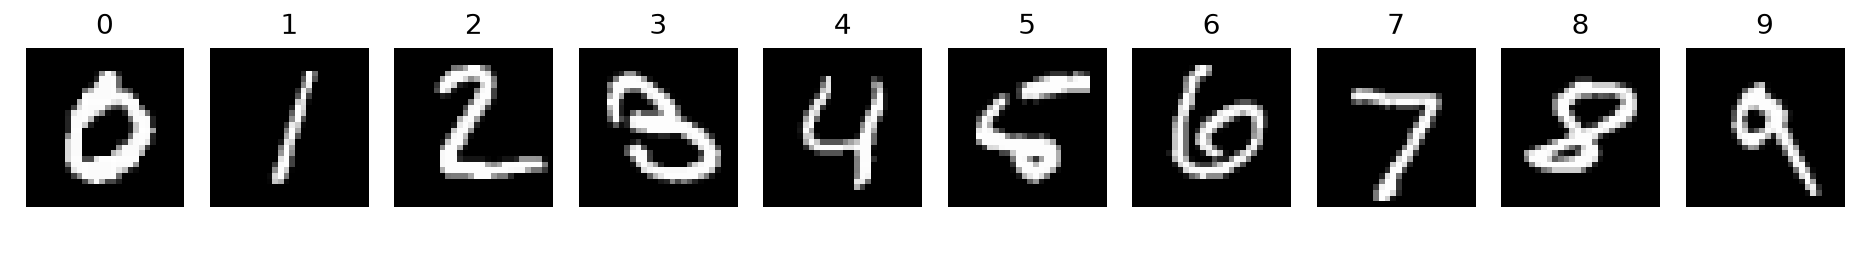
\includegraphics[width=\textwidth]{mnist.png}\par\raggedright\begin{itemize}
\item Dez classes: dígitos de 0 a 9, em imagens em tons de cinza com rótulos conhecidos.
\item As partições originais contêm 60.000 imagens de treino e 10.000 de teste.
\item Verificamos os arquivos baixados e interpretamos o formato IDX.
\end{itemize}
\scriptsize Dataset: LeCun, Cortes e Burges. As imagens são exemplos reais do teste.\note{Ritmo: 50 segundos. Introduza o dataset apenas agora; identifique classes e entrada em tons de cinza.}
\end{frame}

\begin{frame}{Achatamento e normalização}
\[28\times28=784,\qquad x_j=\frac{\mathrm{pixel}_j}{255}\in[0,1]\]\begin{itemize}
\item Convertemos os pixels para float32 e lemos as linhas em ordem fixa.
\item As entradas têm formato (N, 784); os rótulos inteiros têm formato (N,).
\item A MLP recebe valores em posições fixas, sem uma operação própria de vizinhança espacial.
\end{itemize}
\note{Ritmo: 60 segundos. Explique a ordem de leitura por linhas e a divisão fixa por 255.}
\end{frame}

\begin{frame}{Distribuição das classes}
\centering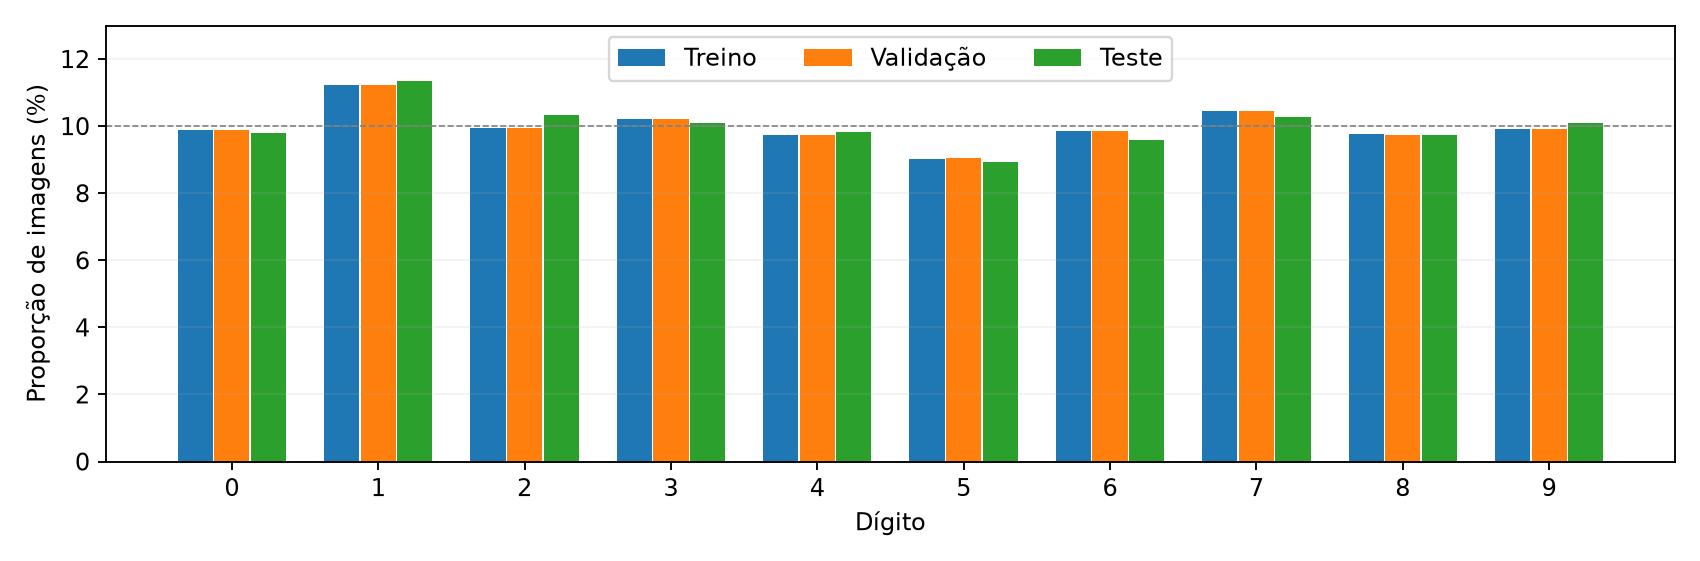
\includegraphics[width=.93\textwidth]{classes_pt.png}\par\raggedright \begin{itemize}
\item As dez classes estão presentes; as proporções são próximas, mas não idênticas à distribuição uniforme.
\item A validação preserva as proporções das classes do treino original.
\end{itemize}

\note{60 segundos. Explique que são porcentagens: os tamanhos dos conjuntos diferem. Contagens exatas em class_counts.json.}
\end{frame}

\begin{frame}{Treino, validação e teste}
\begin{center}\begin{tabular}{lrl}\toprule Partição & Imagens & Finalidade\\\midrule Treino & 50.000 & Atualizar pesos\\ Validação & 10.000 & Selecionar configurações e modelo\\ Teste oficial & 10.000 & Avaliar após a seleção\\\bottomrule\end{tabular}\end{center}\begin{itemize}
\item Dividimos apenas o treino original, com estratificação e seed 42.
\item Usamos apenas normalização: sem correção de inclinação nem aumento de dados nesta execução.
\end{itemize}
\note{Ritmo: 70 segundos. Descreva a estratificação, a seed 42 e por que o teste oficial não orienta a seleção.}
\end{frame}

\section{Parte 3: Implementação, treino e resultados}
\begin{frame}{Nossa arquitetura}
\[784\;\longrightarrow\;128\;\longrightarrow\;64\;\longrightarrow\;10\]\begin{itemize}
\item Duas camadas densas escondidas com ReLU; a saída linear retorna dez logits.
\item 109.386 parâmetros treináveis, incluindo vieses.
\item Os pesos da saída usam Xavier; os pesos escondidos usam He.
\end{itemize}
\[(784\cdot128+128)+(128\cdot64+64)+(64\cdot10+10)=109386\]\[\sigma_{\mathrm{hidden}}=\sqrt{2/n_{\mathrm{in}}},\quad\sigma_{\mathrm{out}}=\sqrt{2/(n_{\mathrm{in}}+n_{\mathrm{out}})},\quad b=0\]\note{Ritmo: 75 segundos. Conecte as equações gerais a 784, 128, 64 e 10; defina a variância de He e Xavier na saída.}
\end{frame}

\begin{frame}{Como organizamos a implementação}
\begin{tabular}{p{.35\textwidth}p{.58\textwidth}}\toprule Módulo & Responsabilidade\\\midrule \texttt{data/mnist.py} & Baixar, verificar, normalizar e dividir\\\texttt{layers.py, activations.py} & Operações vetorizadas de propagação direta e retropropagação\\\texttt{network.py, losses.py} & Compor a MLP e calcular entropia cruzada estável\\\texttt{optimizers.py, trainer.py} & Atualizar parâmetros e coordenar o treino\\\texttt{metrics.py, reporting.py} & Medir e visualizar previsões\\\bottomrule\end{tabular}\par\medskip Pacote: \texttt{src/mnist\_mlp/}. NumPy calcula os gradientes; não usamos frameworks de deep learning.
\note{45 segundos. Mostre a separação de responsabilidades sem listar todo o código.}
\end{frame}

\begin{frame}{SGD com mini-lotes}
\[\theta_{t+1}=\theta_t-\eta\nabla_{\theta}L_{\mathrm{batch}}\]\begin{itemize}
\item Usamos taxa de aprendizado 0,1 e lotes de 64, incluindo o último lote menor.
\item Embaralhamos a ordem do treino a cada época.
\item Uma época é uma passagem completa pelos exemplos de treino.
\item Executamos 20 épocas; a seed 42 controla inicialização, divisão e embaralhamento.
\end{itemize}
\note{Ritmo: 90 segundos. Conecte a regra à taxa 0,1, aos lotes de 64 e ao último lote menor.}
\end{frame}

\begin{frame}{Nosso ciclo de treinamento}
\begin{itemize}
\item Para cada lote: propagação direta, perda, retropropagação e atualização SGD.
\item No fim da época: recalculamos métricas de treino e validação ponderadas por amostra.
\item Salvamos o modelo com a menor perda de validação.
\item Congelamos a seleção antes de medir o desempenho no teste oficial.
\end{itemize}
\small\texttt{data/mnist.py} $\to$ \texttt{network.py} $\to$ \texttt{trainer.py} $\to$ \texttt{evaluate.py}\note{Ritmo: 60 segundos. Selecionamos o melhor checkpoint, sem parada antecipada: todas as 20 épocas são executadas.}
\end{frame}

\begin{frame}{Perda e acurácia ao longo do treino}
\centering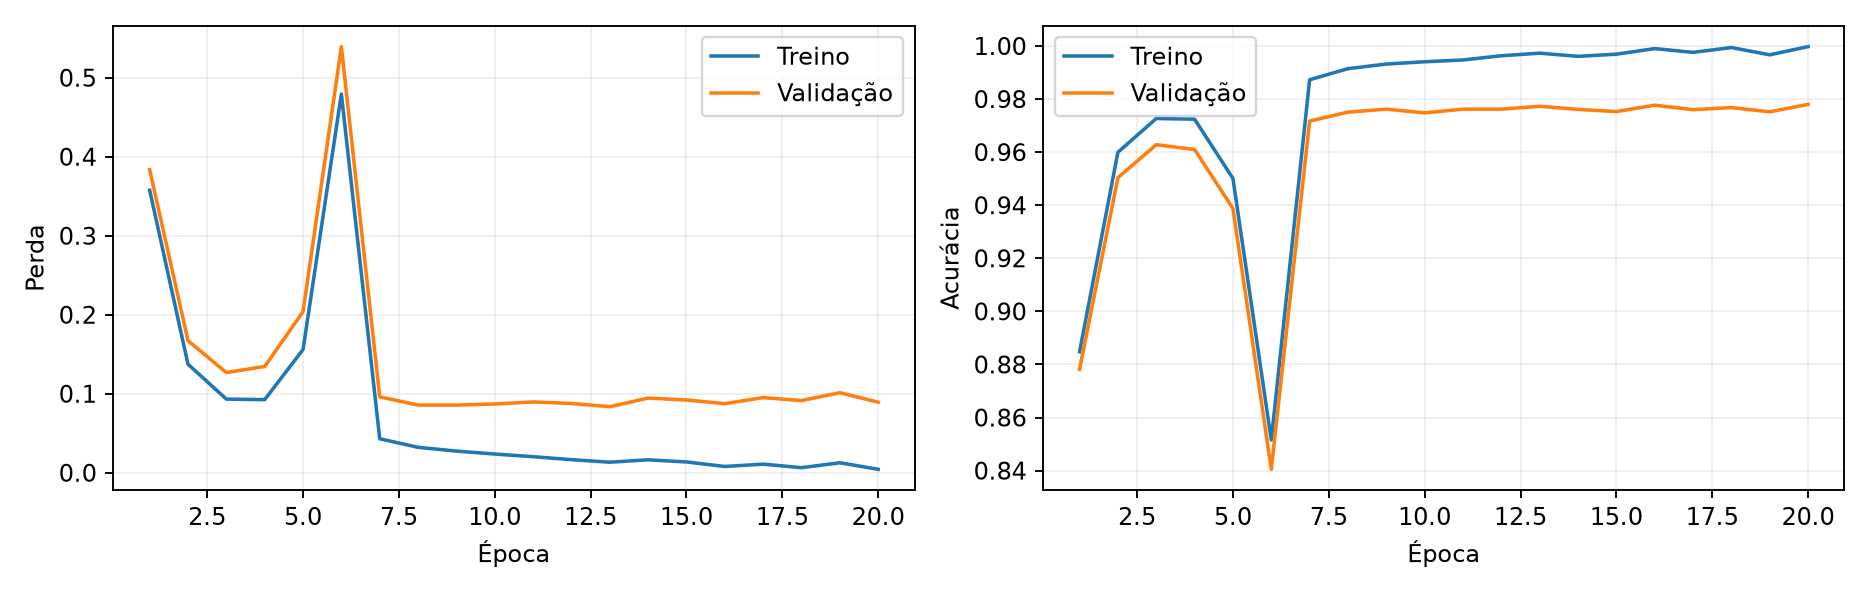
\includegraphics[width=.94\textwidth]{curves_pt.png}\par\raggedright\begin{itemize}
\item A menor perda de validação ocorreu na época 13: 0,083610; acurácia de 97,73\%.
\item Melhorias posteriores no treino não reduziram consistentemente a perda de validação.
\end{itemize}
\note{Ritmo: 80 segundos. Explique os picos temporários e a diferença entre treino e validação; a época 13 vence pela perda de validação.}
\end{frame}

\begin{frame}{Avaliação final do modelo selecionado}
\begin{center}\begin{tabular}{lr}\toprule Métrica de teste & Resultado medido\\\midrule Acurácia & 97,90\%\\ Acertos / erros & 9.790 / 210\\ Entropia cruzada & 0,072777\\ Precisão / revocação macro & 97,90\% / 97,87\%\\ F1 macro / ponderado & 97,88\% / 97,90\%\\ ROC AUC macro / micro & 0,999621 / 0,999617\\\bottomrule\end{tabular}\end{center}Uma execução, uma seed, 10.000 imagens oficiais de teste.\par\scriptsize\texttt{results/baseline/extended\_metrics.json}\note{Ritmo: 65 segundos. Leia acurácia e F1 e diferencie métricas de decisão da AUC de ranking.}
\end{frame}

\begin{frame}{Matriz de confusão}
\begin{columns}[c]\column{.53\textwidth}\centering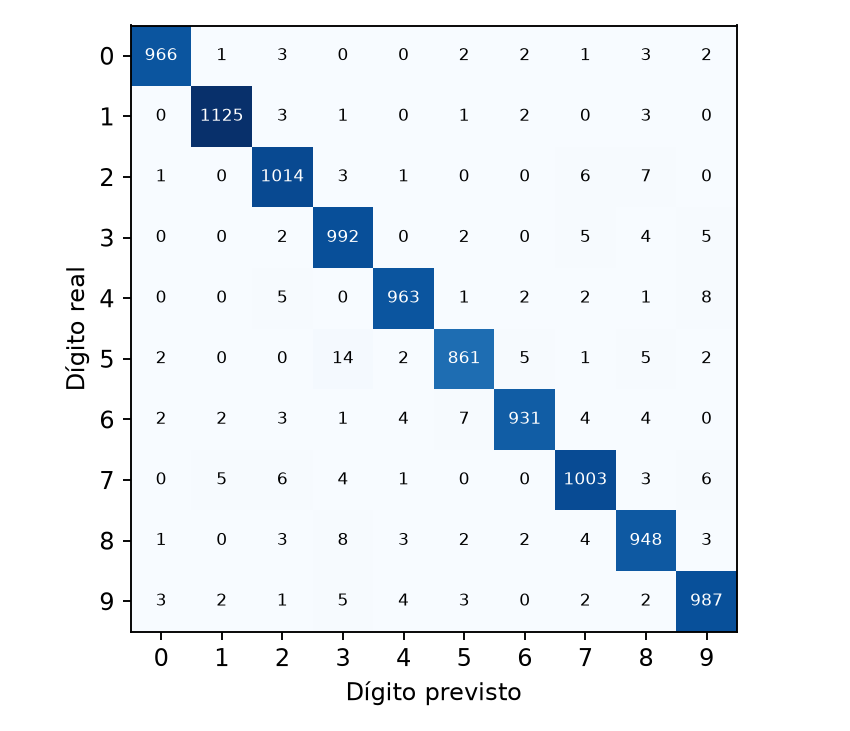
\includegraphics[width=\linewidth,height=.65\textheight,keepaspectratio]{confusion_pt.png}\column{.45\textwidth}\begin{itemize}
\item Linhas são dígitos reais; colunas são previsões.
\item Erro direcionado mais frequente: 5 previsto como 3, com 14 casos.
\item O dígito 8 teve o menor F1: 97,03\%.
\end{itemize}
\end{columns}\note{Ritmo: 55 segundos. Leia uma linha e destaque os 14 casos de cinco previsto como três.}
\end{frame}

\begin{frame}{Curvas ROC e AUC um contra os demais}
\begin{columns}[c]\column{.53\textwidth}\centering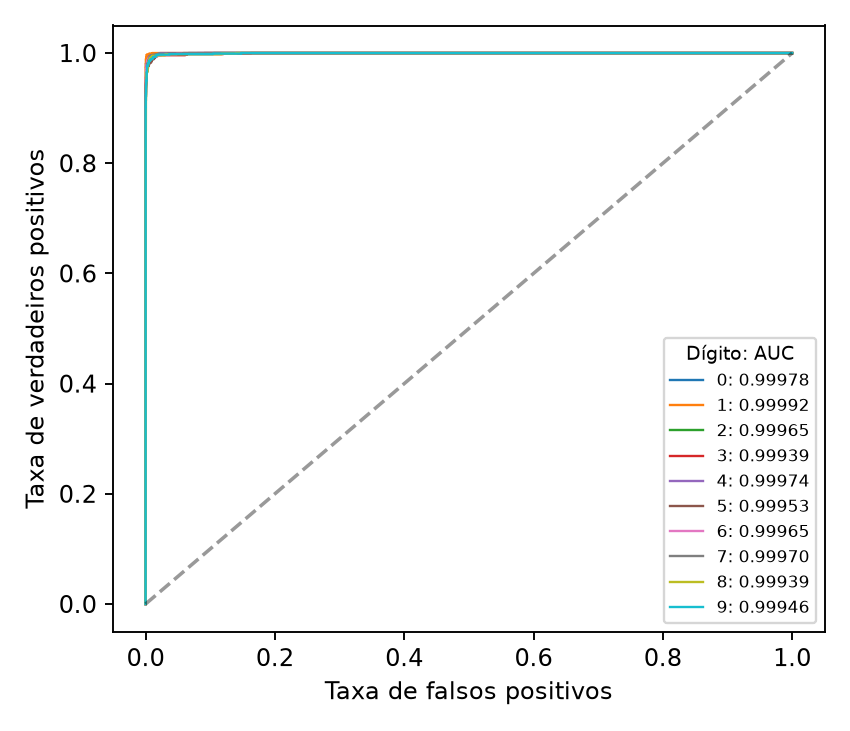
\includegraphics[width=\linewidth,height=.65\textheight,keepaspectratio]{roc_pt.png}\column{.45\textwidth}\begin{itemize}
\item Para cada dígito, variamos um limiar sobre seu escore contra os demais.
\item Macro calcula a média das dez AUCs; micro reúne os pares imagem/classe.
\item AUC alta de ranking não equivale à acurácia multiclasse nem à calibração.
\end{itemize}
\end{columns}\note{Ritmo: 65 segundos. Defina os limiares um contra os demais; AUC próxima de um não significa acurácia multiclasse perfeita.}
\end{frame}

\begin{frame}{Erros reais e previsões confiantes}
\centering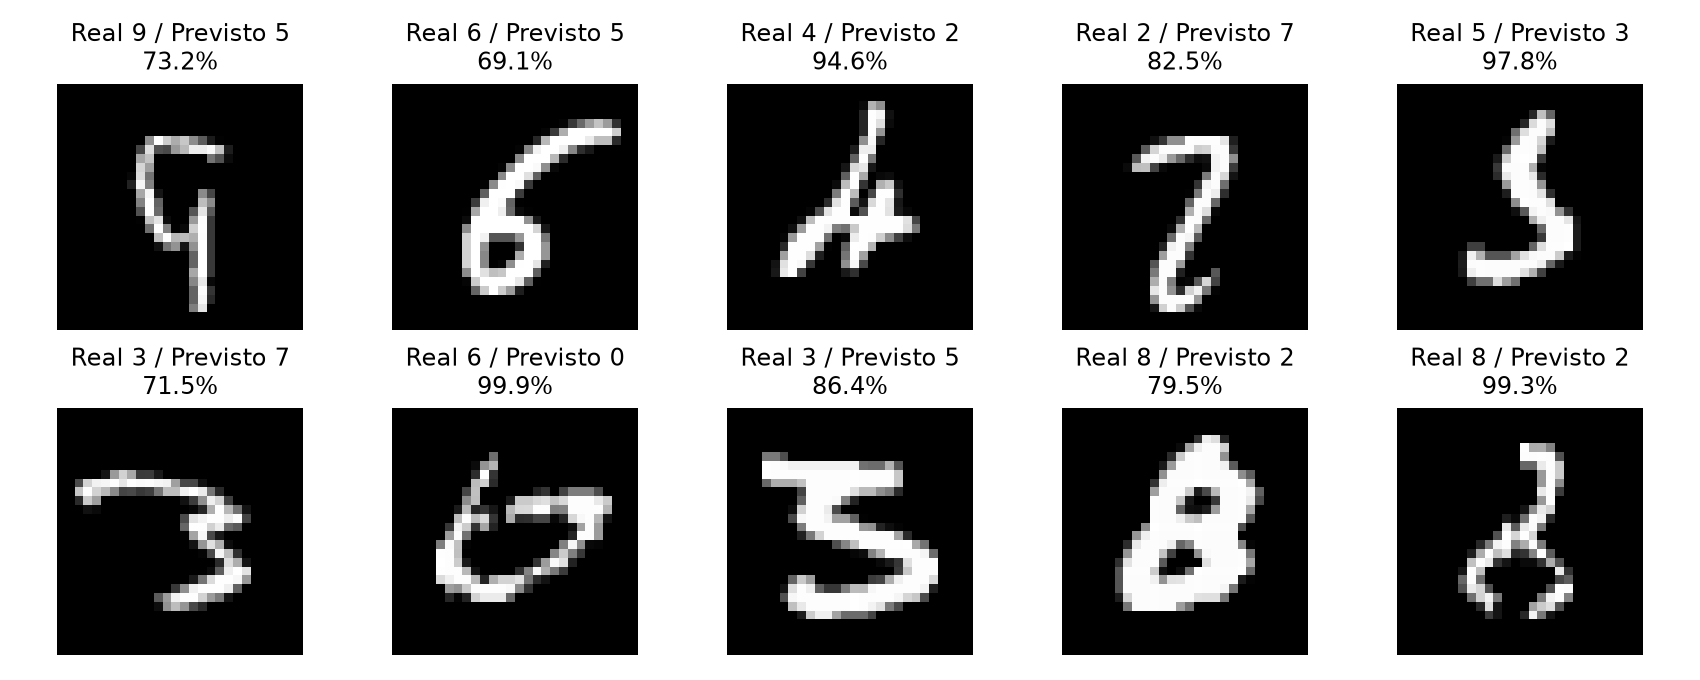
\includegraphics[width=.92\textwidth,height=.61\textheight,keepaspectratio]{errors_pt.png}\par\raggedright Primeiros dez erros na ordem do teste, sem seleção manual. Os valores são escores Softmax da classe prevista.\note{Ritmo: 45 segundos. Explique a seleção determinística dos primeiros dez erros e os escores não calibrados.}
\end{frame}

\begin{frame}{Verificação e limitações}
\begin{itemize}
\item 24 testes cobrem gradientes por diferenças finitas, perda estável, empates na ROC, salvamento e treino.
\item O intervalo de Wilson de 95\% para acurácia é 97,60--98,16\%, sob hipótese binomial, para o modelo fixo.
\item Uma seed não estabelece a variação entre execuções; as saídas Softmax não foram calibradas.
\item Compararíamos seeds, ajustes da taxa e regularização nos dados de validação.
\end{itemize}
\note{Ritmo: 85 segundos. Conclua com gradientes verificados, incerteza de uma seed e futuros experimentos de validação. Reserve cerca de três minutos para discussão na versão principal.}
\end{frame}

\end{document}
